% results.tex -- every results exhibit (tables + figures), input-ready:
% % results.tex -- every results exhibit (tables + figures), input-ready:
% % results.tex -- every results exhibit (tables + figures), input-ready:
% % results.tex -- every results exhibit (tables + figures), input-ready:
% \input{results} from any manuscript. No preamble, no sectioning.
% Requires: booktabs, threeparttable, graphicx, amsmath, and \se macro
% (\newcommand{\se}[1]{{\scriptsize$\pm$#1}}).

\begin{table}[h]
\centering
\begin{threeparttable}
\caption{Net return (\%) by trade year, mean over $V1$--$V4$, 10 seeds.
ONE-NAS books restarted at each window boundary; the 2022--24 column is
one book run over the three-year window.}
\label{tab:window}
\begin{tabular}{lrrrr}
\toprule
 & 2022 & 2023 & 2024 & 2022--24 \\
\midrule
ONE-NAS (40 isl., sleeves book)              & $+6.1$\se{0.8}  & $+12.4$\se{0.7} & $+6.4$\se{0.5}  & $+27.5$\se{1.1} \\
ONE-NAS (40 isl., banded book)\tnote{a}      & $+12.5$\se{1.2} & $+14.6$\se{1.3} & $+3.4$\se{0.9}  & $+33.9$\se{1.8} \\
ONE-NAS (40 isl., Algorithm 1 book)\tnote{b} & $+1.3$\se{1.6}  & $+12.8$\se{1.0} & $+10.8$\se{1.2} & $+25.0$\se{1.8} \\
\midrule
ONE-NAS single champion (8 isl., sleeves)\tnote{c} & $+3.1$\se{1.8} & $+1.7$\se{1.3} & $+2.7$\se{1.1} & $+8.5$ \\
Online LSTM                                  & $+1.2$\se{1.3}  & $+4.5$\se{1.2}  & $+3.8$\se{0.7}  & $+11.3$\se{1.8} \\
Online GRU                                   & $+2.1$\se{1.0}  & $+3.1$\se{1.9}  & $+5.0$\se{0.8}  & $+11.7$\se{2.2} \\
Periodic LSTM (monthly retrain)              & $+1.4$\se{1.0}  & $+3.9$\se{0.8}  & $+6.9$\se{0.6}  & $+14.8$\se{1.0} \\
Online AR\tnote{d}                           & $-14.6$         & $+4.8$          & $+7.9$          & $-3.3$ \\
\midrule
Buy \& hold\tnote{e}                         & $-10.1$         & $+11.2$         & $+6.8$          & $+7.9$ \\
\bottomrule
\end{tabular}
\begin{tablenotes}\footnotesize
\item[a] Buy/hold-spread rule (enter rank $\le$10, exit past 35);
sensitivity row, not an adopted headline.
\item[b] Conditional long--short book (rebalance only when all top-10
predictions are positive and all bottom-10 negative); on rank-normal
predictions the gate fires daily.
\item[c] Published ONE-NAS prediction rule; seeds 42--44 ($n{=}3$).
\item[d] Deterministic; one run per panel. All baselines trade the sleeves
book under identical costs.
\item[e] Equal-weight, prior-study benchmark convention; 2022--24 column
is the sum of yearly cells.
\end{tablenotes}
\end{threeparttable}
\end{table}

\begin{figure}[h]
\centering
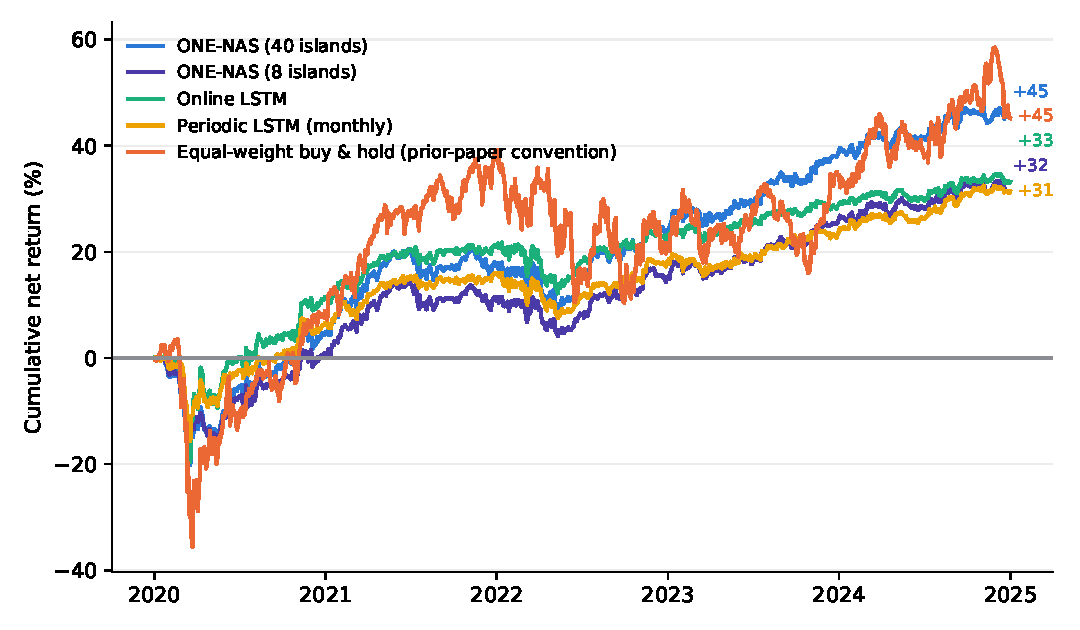
\includegraphics[width=\linewidth]{net_curves.pdf}
\caption{Cumulative net return, 2022--2024 (books restarted at window
start). Buy-and-hold follows the prior paper's benchmark convention.}
\label{fig:curves}
\end{figure}

\begin{table}[h]
\centering
\begin{threeparttable}
\caption{Prediction rule, within-run paired: single global-best genome
vs.\ island-champion rank-mean ensemble from the same runs (sleeves book).
Net \% / Sharpe; $\Delta$ = ensemble $-$ single, paired $t$ over seeds.}
\label{tab:m1}
\begin{tabular}{llrrrr}
\toprule
Fleet & Window & Single & Ensemble & $\Delta$net ($t$) & $\Delta$Sharpe ($t$) \\
\midrule
40 isl.\ ($n{=}10$) & 2022--24 & $+4.5$ / $0.21$  & $+27.5$ / $0.87$ & $+23.0$ $(18.2)$ & $+0.66$ $(14.7)$ \\
40 isl.\ ($n{=}10$) & 2020--24 & $+2.7$ / $0.08$  & $+45.6$ / $0.68$ & $+42.9$ $(14.6)$ & $+0.60$ $(13.4)$ \\
8 isl.\ ($n{=}10$)  & 2022--24 & $+8.3$ / $0.33$  & $+20.5$ / $0.70$ & $+12.2$ $(6.7)$  & $+0.37$ $(5.8)$ \\
8 isl.\ ($n{=}10$)  & 2020--24 & $+12.0$ / $0.21$ & $+32.1$ / $0.52$ & $+20.1$ $(5.5)$  & $+0.30$ $(5.3)$ \\
\midrule
8 isl.\ ($n{=}5$)\tnote{a}  & 2016--19 & $+16.3$ / $0.56$ & $+26.0$ / $0.92$ & $+9.7$ $(5.2)$   & $+0.36$ $(4.5)$ \\
40 isl.\ ($n{=}5$)\tnote{a} & 2016--19 & $+8.9$ / $0.30$  & $+36.7$ / $1.22$ & $+27.8$ $(7.5)$  & $+0.92$ $(6.6)$ \\
\bottomrule
\end{tabular}
\begin{tablenotes}\footnotesize
\item[a] Replication on the 2016--2019 tuning-span fleets.
\end{tablenotes}
\end{threeparttable}
\end{table}

\begin{figure}[h]
\centering
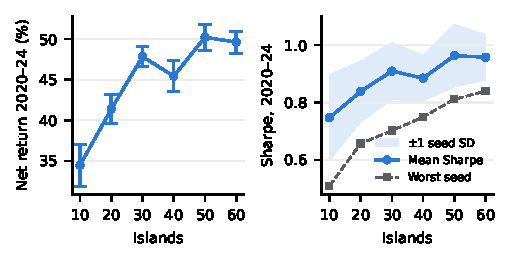
\includegraphics[width=\linewidth]{islands_scaling.pdf}
\caption{Performance vs.\ island count (2020--2024, registered sleeves
book; 10 seeds $\times$ 4 panels at every width). Left: pooled net return
(mean $\pm$ SE). Right: Sharpe --- mean with $\pm$1 seed-SD band, and the
worst seed. Return and Sharpe climb steeply to about 30 islands and then
sit on a plateau ($+45$ to $+50$ net, Sharpe $0.88$--$0.96$) whose widths
are not separable at this replication; the worst seed improves
monotonically across the whole range ($0.51 \to 0.84$) while the seed SD
falls ($0.149 \to 0.079$), so width keeps buying reliability after it
stops buying mean return. The 40-island setting was fixed on the
2016--2019 tuning span before this curve was measured; the nominally
higher 50- and 60-island cells are eval-span measurements and are not
adopted.}
\label{fig:islands}
\end{figure}

\begin{table}[h]
\centering
\begin{threeparttable}
\caption{Paired significance for the 2022--2024 window table: within-cell
difference in net return between ONE-NAS (40 islands) and each other arm,
over the (panel, seed) cells the two share.}
\label{tab:paired}
\begin{tabular}{lrr}
\toprule
Comparison & $\Delta$net & paired $t$ \\
\midrule
vs.\ ONE-NAS (8 isl.)            & $+7.0$  & $3.49$ \\
vs.\ Online LSTM                 & $+16.2$ & $7.32$ \\
vs.\ Online GRU                  & $+15.8$ & $6.59$ \\
vs.\ Periodic LSTM (monthly)     & $+12.7$ & $6.66$ \\
vs.\ Online AR\tnote{a}          & $+34.9$ & $2.22$ \\
\bottomrule
\end{tabular}
\begin{tablenotes}\footnotesize
\item Every comparison is over all 40 (panel, seed) cells unless noted.
Buy \& hold trades once and is not seed-paired, so no paired test is
reported against it.
\item[a] Deterministic; one run per panel, so $n{=}4$.
\end{tablenotes}
\end{threeparttable}
\end{table}

\begin{table}[h]
\centering
\begin{threeparttable}
\caption{Cost sensitivity: net return (\%) on 2022--2024 as the realised
per-name transaction cost is scaled by the stated multiple. The
$1\times$ column is the sleeves-book column of the window table.}
\label{tab:costs}
\begin{tabular}{lrrrrr}
\toprule
Arm & $1\times$ & $2\times$ & $3\times$ & $5\times$ & B/E\tnote{a} \\
\midrule
ONE-NAS (40 isl.)            & $+27.5$ & $+24.7$ & $+21.8$ & $+16.0$ & $10.6\times$ \\
ONE-NAS (8 isl.)             & $+20.5$ & $+17.4$ & $+14.4$ & $+8.2$  & $7.7\times$ \\
Periodic LSTM (monthly)      & $+14.8$ & $+11.4$ & $+8.0$  & $+1.2$  & $5.4\times$ \\
Online GRU                   & $+11.7$ & $+8.3$  & $+4.9$  & $-1.8$  & $4.5\times$ \\
Online LSTM                  & $+11.3$ & $+8.1$  & $+4.9$  & $-1.5$  & $4.5\times$ \\
Online AR                    & $-3.3$  & $-6.0$  & $-8.8$  & $-14.2$ & --- \\
\bottomrule
\end{tabular}
\begin{tablenotes}\footnotesize
\item Scaling multiplies the realised per-name cost, so the
cross-sectional shape of costs is preserved and wide-spread names stay
the expensive ones.
\item[a] Break-even: the cost multiple at which net return reaches zero.
\end{tablenotes}
\end{threeparttable}
\end{table}

\begin{table}[h]
\centering
\caption{Factor-adjusted alphas: pooled daily book returns regressed on
Fama--French three factors plus momentum, 2020--2024, Newey--West lag 10.}
\label{tab:alphas}
\begin{tabular}{lrrrr}
\toprule
Arm & $\alpha$ (bps/day) & $\alpha$ (\%/yr) & NW $t$ & Mkt.\ beta \\
\midrule
ONE-NAS (40 islands)     & $+3.15$ & $+7.9$ & $+2.14$ & $+0.120$ \\
ONE-NAS (8 islands)      & $+2.17$ & $+5.5$ & $+1.76$ & $+0.096$ \\
Periodic LSTM (monthly)  & $+2.15$ & $+5.4$ & $+1.78$ & $+0.079$ \\
Online LSTM              & $+2.08$ & $+5.2$ & $+1.59$ & $+0.130$ \\
Online GRU               & $+1.52$ & $+3.8$ & $+1.35$ & $+0.119$ \\
Online AR                & $-1.35$ & $-3.4$ & $-1.05$ & $+0.007$ \\
\bottomrule
\end{tabular}
\end{table}

\begin{table}[h]
\centering
\caption{Ensemble diversity mechanism: measured member rank IC, pairwise
member prediction correlation $\rho$, measured ensemble IC, and the
equicorrelated averaging prediction $m\sqrt{N/(1+(N-1)\rho)}$.}
\label{tab:diversity}
\begin{tabular}{lccccc}
\toprule
Fleet & $N$ & $\rho$ & Member IC & Ensemble IC & Predicted \\
\midrule
8 isl., 2020--24  & 8  & 0.216 & $+0.0064$ & $+0.0110$ & $+0.0114$ \\
40 isl., 2020--24 & 40 & 0.172 & $+0.0058$ & $+0.0128$ & $+0.0132$ \\
8 isl., 2016--19  & 8  & 0.190 & $+0.0071$ & $+0.0132$ & $+0.0132$ \\
40 isl., 2016--19 & 40 & 0.187 & $+0.0078$ & $+0.0166$ & $+0.0171$ \\
\bottomrule
\end{tabular}
\end{table}

\begin{table}[h]
\centering
\begin{threeparttable}
\caption{Ensembling gain (ensemble $-$ single champion, within-run, net \%
on 2016--2019) inside every trained hyperparameter configuration; positive
in 16/16 cells.}
\label{tab:invariance}
\begin{tabular}{lr@{\qquad}lr}
\toprule
Configuration & $\Delta$net & Configuration & $\Delta$net \\
\midrule
C0 (registered primary) & $+3.9$  & NTS 600            & $+12.8$ \\
Select: IC-gated        & $+0.5$  & Rounds 2           & $+11.0$ \\
Select: IC              & $+2.8$  & PER $\alpha$ 0.4   & $+4.0$  \\
Target: 5-day CS        & $+4.5$  & PER $\alpha$ 0.8   & $+11.7$ \\
5-day CS + IC-gated     & $+1.8$  & PER $\lambda{\times}3$ & $+20.6$ \\
Elite 5 / gen 10        & $+9.6$  & BP epochs 20       & $+12.5$ \\
Elite 5 / gen 15        & $+11.1$ & Repop.\ 25         & $+7.0$  \\
Repop.\ 100             & $+9.6$  & PER off (uniform)  & $+9.3$  \\
\bottomrule
\end{tabular}
\begin{tablenotes}\footnotesize
\item Mean $+8.3$; $n{=}6$ runs per cell (2 panels $\times$ 3 seeds).
\end{tablenotes}
\end{threeparttable}
\end{table}

\begin{table}[h]
\centering
\caption{Online continuity: pooled net (\%) on 2022--2024, frozen 8-island
configuration.}
\label{tab:continuity}
\begin{tabular}{lr}
\toprule
Population evolving online since 2020-01 & $+26.5$ \\
Cold start at 2022-01                     & $+12.3$ \\
\bottomrule
\end{tabular}
\end{table}

\begin{table}[h]
\centering
\caption{ONE-NAS hyperparameter settings (selected on 2016--2019
validation data, disjoint from the evaluation span). Replay sampling
ablated: PER vs.\ uniform shows no advantage on the tuning objective
($\Delta$IC $-0.0024$, $t{=}-1.9$).}
\label{tab:hps}
\begin{tabular}{ll}
\toprule
Hyperparameter & Value \\
\midrule
Islands & 40 (headline); 8 (registered primary) \\
Elite population per island & 8 \\
Generated genomes per island per generation & 5 \\
Repopulation frequency & every 50 generations \\
Selection metric & validation MSE \\
Prediction rule & rank-mean ensemble of island champions \\
Target & 1-day cross-sectional rank-normal return \\
Sequence length / window step / validation sets & 40 / 5 / 5 \\
Training subsequences per genome & 2000 \\
Backpropagation epochs per genome & 10 \\
Replay (PER) $\alpha$, $\lambda$, $\epsilon$ & 0.6, 0.007, $10^{-8}$ \\
Rounds per generation & 1 \\
Node-type library & simple, UGRNN, MGU, GRU, $\Delta$-RNN, LSTM \\
Mutation / intra- / inter-island crossover & 0.7 / 0.2 / 0.1 (framework defaults) \\
Warm-up generations & 50 \\
\bottomrule
\end{tabular}
\end{table}
 from any manuscript. No preamble, no sectioning.
% Requires: booktabs, threeparttable, graphicx, amsmath, and \se macro
% (\newcommand{\se}[1]{{\scriptsize$\pm$#1}}).

\begin{table}[h]
\centering
\begin{threeparttable}
\caption{Net return (\%) by trade year, mean over $V1$--$V4$, 10 seeds.
ONE-NAS books restarted at each window boundary; the 2022--24 column is
one book run over the three-year window.}
\label{tab:window}
\begin{tabular}{lrrrr}
\toprule
 & 2022 & 2023 & 2024 & 2022--24 \\
\midrule
ONE-NAS (40 isl., sleeves book)              & $+6.1$\se{0.8}  & $+12.4$\se{0.7} & $+6.4$\se{0.5}  & $+27.5$\se{1.1} \\
ONE-NAS (40 isl., banded book)\tnote{a}      & $+12.5$\se{1.2} & $+14.6$\se{1.3} & $+3.4$\se{0.9}  & $+33.9$\se{1.8} \\
ONE-NAS (40 isl., Algorithm 1 book)\tnote{b} & $+1.3$\se{1.6}  & $+12.8$\se{1.0} & $+10.8$\se{1.2} & $+25.0$\se{1.8} \\
\midrule
ONE-NAS single champion (8 isl., sleeves)\tnote{c} & $+3.1$\se{1.8} & $+1.7$\se{1.3} & $+2.7$\se{1.1} & $+8.5$ \\
Online LSTM                                  & $+1.2$\se{1.3}  & $+4.5$\se{1.2}  & $+3.8$\se{0.7}  & $+11.3$\se{1.8} \\
Online GRU                                   & $+2.1$\se{1.0}  & $+3.1$\se{1.9}  & $+5.0$\se{0.8}  & $+11.7$\se{2.2} \\
Periodic LSTM (monthly retrain)              & $+1.4$\se{1.0}  & $+3.9$\se{0.8}  & $+6.9$\se{0.6}  & $+14.8$\se{1.0} \\
Online AR\tnote{d}                           & $-14.6$         & $+4.8$          & $+7.9$          & $-3.3$ \\
\midrule
Buy \& hold\tnote{e}                         & $-10.1$         & $+11.2$         & $+6.8$          & $+7.9$ \\
\bottomrule
\end{tabular}
\begin{tablenotes}\footnotesize
\item[a] Buy/hold-spread rule (enter rank $\le$10, exit past 35);
sensitivity row, not an adopted headline.
\item[b] Conditional long--short book (rebalance only when all top-10
predictions are positive and all bottom-10 negative); on rank-normal
predictions the gate fires daily.
\item[c] Published ONE-NAS prediction rule; seeds 42--44 ($n{=}3$).
\item[d] Deterministic; one run per panel. All baselines trade the sleeves
book under identical costs.
\item[e] Equal-weight, prior-study benchmark convention; 2022--24 column
is the sum of yearly cells.
\end{tablenotes}
\end{threeparttable}
\end{table}

\begin{figure}[h]
\centering
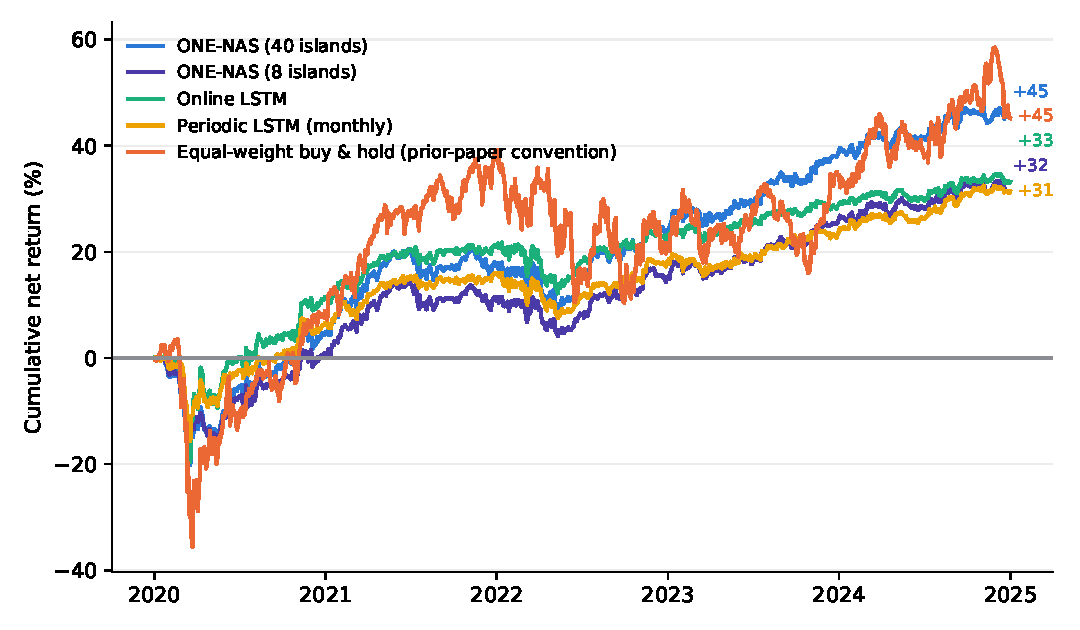
\includegraphics[width=\linewidth]{net_curves.pdf}
\caption{Cumulative net return, 2022--2024 (books restarted at window
start). Buy-and-hold follows the prior paper's benchmark convention.}
\label{fig:curves}
\end{figure}

\begin{table}[h]
\centering
\begin{threeparttable}
\caption{Prediction rule, within-run paired: single global-best genome
vs.\ island-champion rank-mean ensemble from the same runs (sleeves book).
Net \% / Sharpe; $\Delta$ = ensemble $-$ single, paired $t$ over seeds.}
\label{tab:m1}
\begin{tabular}{llrrrr}
\toprule
Fleet & Window & Single & Ensemble & $\Delta$net ($t$) & $\Delta$Sharpe ($t$) \\
\midrule
40 isl.\ ($n{=}10$) & 2022--24 & $+4.5$ / $0.21$  & $+27.5$ / $0.87$ & $+23.0$ $(18.2)$ & $+0.66$ $(14.7)$ \\
40 isl.\ ($n{=}10$) & 2020--24 & $+2.7$ / $0.08$  & $+45.6$ / $0.68$ & $+42.9$ $(14.6)$ & $+0.60$ $(13.4)$ \\
8 isl.\ ($n{=}10$)  & 2022--24 & $+8.3$ / $0.33$  & $+20.5$ / $0.70$ & $+12.2$ $(6.7)$  & $+0.37$ $(5.8)$ \\
8 isl.\ ($n{=}10$)  & 2020--24 & $+12.0$ / $0.21$ & $+32.1$ / $0.52$ & $+20.1$ $(5.5)$  & $+0.30$ $(5.3)$ \\
\midrule
8 isl.\ ($n{=}5$)\tnote{a}  & 2016--19 & $+16.3$ / $0.56$ & $+26.0$ / $0.92$ & $+9.7$ $(5.2)$   & $+0.36$ $(4.5)$ \\
40 isl.\ ($n{=}5$)\tnote{a} & 2016--19 & $+8.9$ / $0.30$  & $+36.7$ / $1.22$ & $+27.8$ $(7.5)$  & $+0.92$ $(6.6)$ \\
\bottomrule
\end{tabular}
\begin{tablenotes}\footnotesize
\item[a] Replication on the 2016--2019 tuning-span fleets.
\end{tablenotes}
\end{threeparttable}
\end{table}

\begin{figure}[h]
\centering
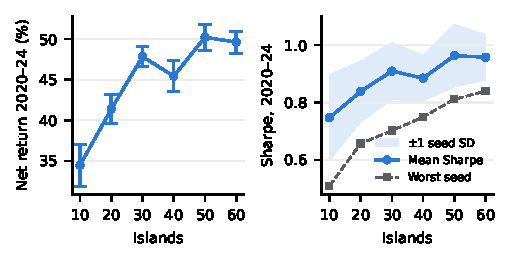
\includegraphics[width=\linewidth]{islands_scaling.pdf}
\caption{Performance vs.\ island count (2020--2024, registered sleeves
book; 10 seeds $\times$ 4 panels at every width). Left: pooled net return
(mean $\pm$ SE). Right: Sharpe --- mean with $\pm$1 seed-SD band, and the
worst seed. Return and Sharpe climb steeply to about 30 islands and then
sit on a plateau ($+45$ to $+50$ net, Sharpe $0.88$--$0.96$) whose widths
are not separable at this replication; the worst seed improves
monotonically across the whole range ($0.51 \to 0.84$) while the seed SD
falls ($0.149 \to 0.079$), so width keeps buying reliability after it
stops buying mean return. The 40-island setting was fixed on the
2016--2019 tuning span before this curve was measured; the nominally
higher 50- and 60-island cells are eval-span measurements and are not
adopted.}
\label{fig:islands}
\end{figure}

\begin{table}[h]
\centering
\begin{threeparttable}
\caption{Paired significance for the 2022--2024 window table: within-cell
difference in net return between ONE-NAS (40 islands) and each other arm,
over the (panel, seed) cells the two share.}
\label{tab:paired}
\begin{tabular}{lrr}
\toprule
Comparison & $\Delta$net & paired $t$ \\
\midrule
vs.\ ONE-NAS (8 isl.)            & $+7.0$  & $3.49$ \\
vs.\ Online LSTM                 & $+16.2$ & $7.32$ \\
vs.\ Online GRU                  & $+15.8$ & $6.59$ \\
vs.\ Periodic LSTM (monthly)     & $+12.7$ & $6.66$ \\
vs.\ Online AR\tnote{a}          & $+34.9$ & $2.22$ \\
\bottomrule
\end{tabular}
\begin{tablenotes}\footnotesize
\item Every comparison is over all 40 (panel, seed) cells unless noted.
Buy \& hold trades once and is not seed-paired, so no paired test is
reported against it.
\item[a] Deterministic; one run per panel, so $n{=}4$.
\end{tablenotes}
\end{threeparttable}
\end{table}

\begin{table}[h]
\centering
\begin{threeparttable}
\caption{Cost sensitivity: net return (\%) on 2022--2024 as the realised
per-name transaction cost is scaled by the stated multiple. The
$1\times$ column is the sleeves-book column of the window table.}
\label{tab:costs}
\begin{tabular}{lrrrrr}
\toprule
Arm & $1\times$ & $2\times$ & $3\times$ & $5\times$ & B/E\tnote{a} \\
\midrule
ONE-NAS (40 isl.)            & $+27.5$ & $+24.7$ & $+21.8$ & $+16.0$ & $10.6\times$ \\
ONE-NAS (8 isl.)             & $+20.5$ & $+17.4$ & $+14.4$ & $+8.2$  & $7.7\times$ \\
Periodic LSTM (monthly)      & $+14.8$ & $+11.4$ & $+8.0$  & $+1.2$  & $5.4\times$ \\
Online GRU                   & $+11.7$ & $+8.3$  & $+4.9$  & $-1.8$  & $4.5\times$ \\
Online LSTM                  & $+11.3$ & $+8.1$  & $+4.9$  & $-1.5$  & $4.5\times$ \\
Online AR                    & $-3.3$  & $-6.0$  & $-8.8$  & $-14.2$ & --- \\
\bottomrule
\end{tabular}
\begin{tablenotes}\footnotesize
\item Scaling multiplies the realised per-name cost, so the
cross-sectional shape of costs is preserved and wide-spread names stay
the expensive ones.
\item[a] Break-even: the cost multiple at which net return reaches zero.
\end{tablenotes}
\end{threeparttable}
\end{table}

\begin{table}[h]
\centering
\caption{Factor-adjusted alphas: pooled daily book returns regressed on
Fama--French three factors plus momentum, 2020--2024, Newey--West lag 10.}
\label{tab:alphas}
\begin{tabular}{lrrrr}
\toprule
Arm & $\alpha$ (bps/day) & $\alpha$ (\%/yr) & NW $t$ & Mkt.\ beta \\
\midrule
ONE-NAS (40 islands)     & $+3.15$ & $+7.9$ & $+2.14$ & $+0.120$ \\
ONE-NAS (8 islands)      & $+2.17$ & $+5.5$ & $+1.76$ & $+0.096$ \\
Periodic LSTM (monthly)  & $+2.15$ & $+5.4$ & $+1.78$ & $+0.079$ \\
Online LSTM              & $+2.08$ & $+5.2$ & $+1.59$ & $+0.130$ \\
Online GRU               & $+1.52$ & $+3.8$ & $+1.35$ & $+0.119$ \\
Online AR                & $-1.35$ & $-3.4$ & $-1.05$ & $+0.007$ \\
\bottomrule
\end{tabular}
\end{table}

\begin{table}[h]
\centering
\caption{Ensemble diversity mechanism: measured member rank IC, pairwise
member prediction correlation $\rho$, measured ensemble IC, and the
equicorrelated averaging prediction $m\sqrt{N/(1+(N-1)\rho)}$.}
\label{tab:diversity}
\begin{tabular}{lccccc}
\toprule
Fleet & $N$ & $\rho$ & Member IC & Ensemble IC & Predicted \\
\midrule
8 isl., 2020--24  & 8  & 0.216 & $+0.0064$ & $+0.0110$ & $+0.0114$ \\
40 isl., 2020--24 & 40 & 0.172 & $+0.0058$ & $+0.0128$ & $+0.0132$ \\
8 isl., 2016--19  & 8  & 0.190 & $+0.0071$ & $+0.0132$ & $+0.0132$ \\
40 isl., 2016--19 & 40 & 0.187 & $+0.0078$ & $+0.0166$ & $+0.0171$ \\
\bottomrule
\end{tabular}
\end{table}

\begin{table}[h]
\centering
\begin{threeparttable}
\caption{Ensembling gain (ensemble $-$ single champion, within-run, net \%
on 2016--2019) inside every trained hyperparameter configuration; positive
in 16/16 cells.}
\label{tab:invariance}
\begin{tabular}{lr@{\qquad}lr}
\toprule
Configuration & $\Delta$net & Configuration & $\Delta$net \\
\midrule
C0 (registered primary) & $+3.9$  & NTS 600            & $+12.8$ \\
Select: IC-gated        & $+0.5$  & Rounds 2           & $+11.0$ \\
Select: IC              & $+2.8$  & PER $\alpha$ 0.4   & $+4.0$  \\
Target: 5-day CS        & $+4.5$  & PER $\alpha$ 0.8   & $+11.7$ \\
5-day CS + IC-gated     & $+1.8$  & PER $\lambda{\times}3$ & $+20.6$ \\
Elite 5 / gen 10        & $+9.6$  & BP epochs 20       & $+12.5$ \\
Elite 5 / gen 15        & $+11.1$ & Repop.\ 25         & $+7.0$  \\
Repop.\ 100             & $+9.6$  & PER off (uniform)  & $+9.3$  \\
\bottomrule
\end{tabular}
\begin{tablenotes}\footnotesize
\item Mean $+8.3$; $n{=}6$ runs per cell (2 panels $\times$ 3 seeds).
\end{tablenotes}
\end{threeparttable}
\end{table}

\begin{table}[h]
\centering
\caption{Online continuity: pooled net (\%) on 2022--2024, frozen 8-island
configuration.}
\label{tab:continuity}
\begin{tabular}{lr}
\toprule
Population evolving online since 2020-01 & $+26.5$ \\
Cold start at 2022-01                     & $+12.3$ \\
\bottomrule
\end{tabular}
\end{table}

\begin{table}[h]
\centering
\caption{ONE-NAS hyperparameter settings (selected on 2016--2019
validation data, disjoint from the evaluation span). Replay sampling
ablated: PER vs.\ uniform shows no advantage on the tuning objective
($\Delta$IC $-0.0024$, $t{=}-1.9$).}
\label{tab:hps}
\begin{tabular}{ll}
\toprule
Hyperparameter & Value \\
\midrule
Islands & 40 (headline); 8 (registered primary) \\
Elite population per island & 8 \\
Generated genomes per island per generation & 5 \\
Repopulation frequency & every 50 generations \\
Selection metric & validation MSE \\
Prediction rule & rank-mean ensemble of island champions \\
Target & 1-day cross-sectional rank-normal return \\
Sequence length / window step / validation sets & 40 / 5 / 5 \\
Training subsequences per genome & 2000 \\
Backpropagation epochs per genome & 10 \\
Replay (PER) $\alpha$, $\lambda$, $\epsilon$ & 0.6, 0.007, $10^{-8}$ \\
Rounds per generation & 1 \\
Node-type library & simple, UGRNN, MGU, GRU, $\Delta$-RNN, LSTM \\
Mutation / intra- / inter-island crossover & 0.7 / 0.2 / 0.1 (framework defaults) \\
Warm-up generations & 50 \\
\bottomrule
\end{tabular}
\end{table}
 from any manuscript. No preamble, no sectioning.
% Requires: booktabs, threeparttable, graphicx, amsmath, and \se macro
% (\newcommand{\se}[1]{{\scriptsize$\pm$#1}}).

\begin{table}[h]
\centering
\begin{threeparttable}
\caption{Net return (\%) by trade year, mean over $V1$--$V4$, 10 seeds.
ONE-NAS books restarted at each window boundary; the 2022--24 column is
one book run over the three-year window.}
\label{tab:window}
\begin{tabular}{lrrrr}
\toprule
 & 2022 & 2023 & 2024 & 2022--24 \\
\midrule
ONE-NAS (40 isl., sleeves book)              & $+6.1$\se{0.8}  & $+12.4$\se{0.7} & $+6.4$\se{0.5}  & $+27.5$\se{1.1} \\
ONE-NAS (40 isl., banded book)\tnote{a}      & $+12.5$\se{1.2} & $+14.6$\se{1.3} & $+3.4$\se{0.9}  & $+33.9$\se{1.8} \\
ONE-NAS (40 isl., Algorithm 1 book)\tnote{b} & $+1.3$\se{1.6}  & $+12.8$\se{1.0} & $+10.8$\se{1.2} & $+25.0$\se{1.8} \\
\midrule
ONE-NAS single champion (8 isl., sleeves)\tnote{c} & $+3.1$\se{1.8} & $+1.7$\se{1.3} & $+2.7$\se{1.1} & $+8.5$ \\
Online LSTM                                  & $+1.2$\se{1.3}  & $+4.5$\se{1.2}  & $+3.8$\se{0.7}  & $+11.3$\se{1.8} \\
Online GRU                                   & $+2.1$\se{1.0}  & $+3.1$\se{1.9}  & $+5.0$\se{0.8}  & $+11.7$\se{2.2} \\
Periodic LSTM (monthly retrain)              & $+1.4$\se{1.0}  & $+3.9$\se{0.8}  & $+6.9$\se{0.6}  & $+14.8$\se{1.0} \\
Online AR\tnote{d}                           & $-14.6$         & $+4.8$          & $+7.9$          & $-3.3$ \\
\midrule
Buy \& hold\tnote{e}                         & $-10.1$         & $+11.2$         & $+6.8$          & $+7.9$ \\
\bottomrule
\end{tabular}
\begin{tablenotes}\footnotesize
\item[a] Buy/hold-spread rule (enter rank $\le$10, exit past 35);
sensitivity row, not an adopted headline.
\item[b] Conditional long--short book (rebalance only when all top-10
predictions are positive and all bottom-10 negative); on rank-normal
predictions the gate fires daily.
\item[c] Published ONE-NAS prediction rule; seeds 42--44 ($n{=}3$).
\item[d] Deterministic; one run per panel. All baselines trade the sleeves
book under identical costs.
\item[e] Equal-weight, prior-study benchmark convention; 2022--24 column
is the sum of yearly cells.
\end{tablenotes}
\end{threeparttable}
\end{table}

\begin{figure}[h]
\centering
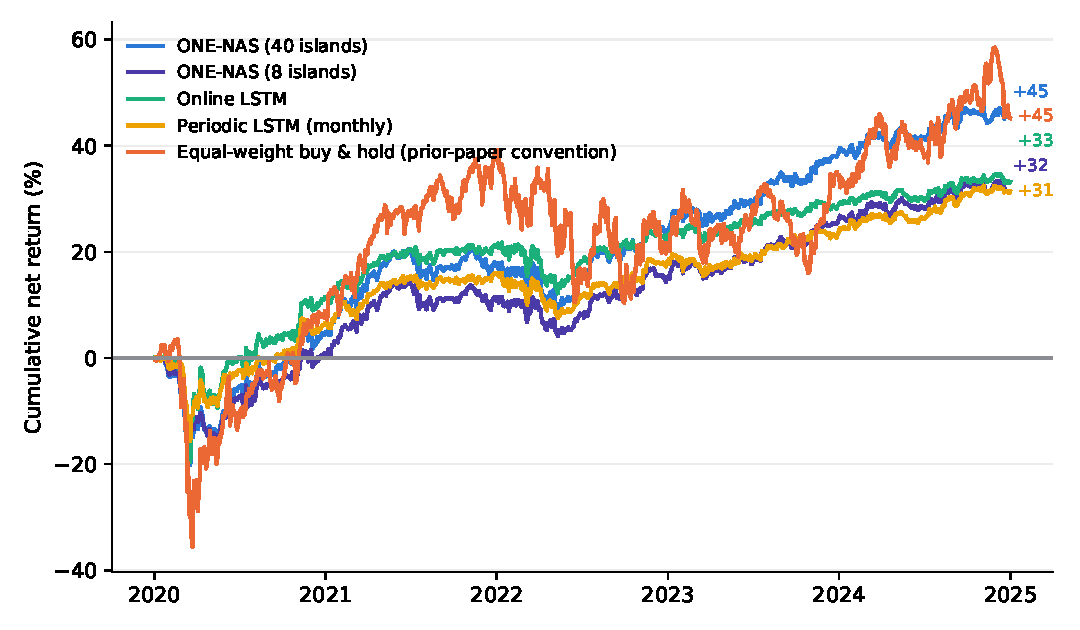
\includegraphics[width=\linewidth]{net_curves.pdf}
\caption{Cumulative net return, 2022--2024 (books restarted at window
start). Buy-and-hold follows the prior paper's benchmark convention.}
\label{fig:curves}
\end{figure}

\begin{table}[h]
\centering
\begin{threeparttable}
\caption{Prediction rule, within-run paired: single global-best genome
vs.\ island-champion rank-mean ensemble from the same runs (sleeves book).
Net \% / Sharpe; $\Delta$ = ensemble $-$ single, paired $t$ over seeds.}
\label{tab:m1}
\begin{tabular}{llrrrr}
\toprule
Fleet & Window & Single & Ensemble & $\Delta$net ($t$) & $\Delta$Sharpe ($t$) \\
\midrule
40 isl.\ ($n{=}10$) & 2022--24 & $+4.5$ / $0.21$  & $+27.5$ / $0.87$ & $+23.0$ $(18.2)$ & $+0.66$ $(14.7)$ \\
40 isl.\ ($n{=}10$) & 2020--24 & $+2.7$ / $0.08$  & $+45.6$ / $0.68$ & $+42.9$ $(14.6)$ & $+0.60$ $(13.4)$ \\
8 isl.\ ($n{=}10$)  & 2022--24 & $+8.3$ / $0.33$  & $+20.5$ / $0.70$ & $+12.2$ $(6.7)$  & $+0.37$ $(5.8)$ \\
8 isl.\ ($n{=}10$)  & 2020--24 & $+12.0$ / $0.21$ & $+32.1$ / $0.52$ & $+20.1$ $(5.5)$  & $+0.30$ $(5.3)$ \\
\midrule
8 isl.\ ($n{=}5$)\tnote{a}  & 2016--19 & $+16.3$ / $0.56$ & $+26.0$ / $0.92$ & $+9.7$ $(5.2)$   & $+0.36$ $(4.5)$ \\
40 isl.\ ($n{=}5$)\tnote{a} & 2016--19 & $+8.9$ / $0.30$  & $+36.7$ / $1.22$ & $+27.8$ $(7.5)$  & $+0.92$ $(6.6)$ \\
\bottomrule
\end{tabular}
\begin{tablenotes}\footnotesize
\item[a] Replication on the 2016--2019 tuning-span fleets.
\end{tablenotes}
\end{threeparttable}
\end{table}

\begin{figure}[h]
\centering
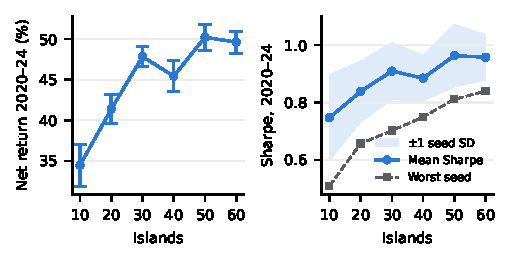
\includegraphics[width=\linewidth]{islands_scaling.pdf}
\caption{Performance vs.\ island count (2020--2024, registered sleeves
book; 10 seeds $\times$ 4 panels at every width). Left: pooled net return
(mean $\pm$ SE). Right: Sharpe --- mean with $\pm$1 seed-SD band, and the
worst seed. Return and Sharpe climb steeply to about 30 islands and then
sit on a plateau ($+45$ to $+50$ net, Sharpe $0.88$--$0.96$) whose widths
are not separable at this replication; the worst seed improves
monotonically across the whole range ($0.51 \to 0.84$) while the seed SD
falls ($0.149 \to 0.079$), so width keeps buying reliability after it
stops buying mean return. The 40-island setting was fixed on the
2016--2019 tuning span before this curve was measured; the nominally
higher 50- and 60-island cells are eval-span measurements and are not
adopted.}
\label{fig:islands}
\end{figure}

\begin{table}[h]
\centering
\begin{threeparttable}
\caption{Paired significance for the 2022--2024 window table: within-cell
difference in net return between ONE-NAS (40 islands) and each other arm,
over the (panel, seed) cells the two share.}
\label{tab:paired}
\begin{tabular}{lrr}
\toprule
Comparison & $\Delta$net & paired $t$ \\
\midrule
vs.\ ONE-NAS (8 isl.)            & $+7.0$  & $3.49$ \\
vs.\ Online LSTM                 & $+16.2$ & $7.32$ \\
vs.\ Online GRU                  & $+15.8$ & $6.59$ \\
vs.\ Periodic LSTM (monthly)     & $+12.7$ & $6.66$ \\
vs.\ Online AR\tnote{a}          & $+34.9$ & $2.22$ \\
\bottomrule
\end{tabular}
\begin{tablenotes}\footnotesize
\item Every comparison is over all 40 (panel, seed) cells unless noted.
Buy \& hold trades once and is not seed-paired, so no paired test is
reported against it.
\item[a] Deterministic; one run per panel, so $n{=}4$.
\end{tablenotes}
\end{threeparttable}
\end{table}

\begin{table}[h]
\centering
\begin{threeparttable}
\caption{Cost sensitivity: net return (\%) on 2022--2024 as the realised
per-name transaction cost is scaled by the stated multiple. The
$1\times$ column is the sleeves-book column of the window table.}
\label{tab:costs}
\begin{tabular}{lrrrrr}
\toprule
Arm & $1\times$ & $2\times$ & $3\times$ & $5\times$ & B/E\tnote{a} \\
\midrule
ONE-NAS (40 isl.)            & $+27.5$ & $+24.7$ & $+21.8$ & $+16.0$ & $10.6\times$ \\
ONE-NAS (8 isl.)             & $+20.5$ & $+17.4$ & $+14.4$ & $+8.2$  & $7.7\times$ \\
Periodic LSTM (monthly)      & $+14.8$ & $+11.4$ & $+8.0$  & $+1.2$  & $5.4\times$ \\
Online GRU                   & $+11.7$ & $+8.3$  & $+4.9$  & $-1.8$  & $4.5\times$ \\
Online LSTM                  & $+11.3$ & $+8.1$  & $+4.9$  & $-1.5$  & $4.5\times$ \\
Online AR                    & $-3.3$  & $-6.0$  & $-8.8$  & $-14.2$ & --- \\
\bottomrule
\end{tabular}
\begin{tablenotes}\footnotesize
\item Scaling multiplies the realised per-name cost, so the
cross-sectional shape of costs is preserved and wide-spread names stay
the expensive ones.
\item[a] Break-even: the cost multiple at which net return reaches zero.
\end{tablenotes}
\end{threeparttable}
\end{table}

\begin{table}[h]
\centering
\caption{Factor-adjusted alphas: pooled daily book returns regressed on
Fama--French three factors plus momentum, 2020--2024, Newey--West lag 10.}
\label{tab:alphas}
\begin{tabular}{lrrrr}
\toprule
Arm & $\alpha$ (bps/day) & $\alpha$ (\%/yr) & NW $t$ & Mkt.\ beta \\
\midrule
ONE-NAS (40 islands)     & $+3.15$ & $+7.9$ & $+2.14$ & $+0.120$ \\
ONE-NAS (8 islands)      & $+2.17$ & $+5.5$ & $+1.76$ & $+0.096$ \\
Periodic LSTM (monthly)  & $+2.15$ & $+5.4$ & $+1.78$ & $+0.079$ \\
Online LSTM              & $+2.08$ & $+5.2$ & $+1.59$ & $+0.130$ \\
Online GRU               & $+1.52$ & $+3.8$ & $+1.35$ & $+0.119$ \\
Online AR                & $-1.35$ & $-3.4$ & $-1.05$ & $+0.007$ \\
\bottomrule
\end{tabular}
\end{table}

\begin{table}[h]
\centering
\caption{Ensemble diversity mechanism: measured member rank IC, pairwise
member prediction correlation $\rho$, measured ensemble IC, and the
equicorrelated averaging prediction $m\sqrt{N/(1+(N-1)\rho)}$.}
\label{tab:diversity}
\begin{tabular}{lccccc}
\toprule
Fleet & $N$ & $\rho$ & Member IC & Ensemble IC & Predicted \\
\midrule
8 isl., 2020--24  & 8  & 0.216 & $+0.0064$ & $+0.0110$ & $+0.0114$ \\
40 isl., 2020--24 & 40 & 0.172 & $+0.0058$ & $+0.0128$ & $+0.0132$ \\
8 isl., 2016--19  & 8  & 0.190 & $+0.0071$ & $+0.0132$ & $+0.0132$ \\
40 isl., 2016--19 & 40 & 0.187 & $+0.0078$ & $+0.0166$ & $+0.0171$ \\
\bottomrule
\end{tabular}
\end{table}

\begin{table}[h]
\centering
\begin{threeparttable}
\caption{Ensembling gain (ensemble $-$ single champion, within-run, net \%
on 2016--2019) inside every trained hyperparameter configuration; positive
in 16/16 cells.}
\label{tab:invariance}
\begin{tabular}{lr@{\qquad}lr}
\toprule
Configuration & $\Delta$net & Configuration & $\Delta$net \\
\midrule
C0 (registered primary) & $+3.9$  & NTS 600            & $+12.8$ \\
Select: IC-gated        & $+0.5$  & Rounds 2           & $+11.0$ \\
Select: IC              & $+2.8$  & PER $\alpha$ 0.4   & $+4.0$  \\
Target: 5-day CS        & $+4.5$  & PER $\alpha$ 0.8   & $+11.7$ \\
5-day CS + IC-gated     & $+1.8$  & PER $\lambda{\times}3$ & $+20.6$ \\
Elite 5 / gen 10        & $+9.6$  & BP epochs 20       & $+12.5$ \\
Elite 5 / gen 15        & $+11.1$ & Repop.\ 25         & $+7.0$  \\
Repop.\ 100             & $+9.6$  & PER off (uniform)  & $+9.3$  \\
\bottomrule
\end{tabular}
\begin{tablenotes}\footnotesize
\item Mean $+8.3$; $n{=}6$ runs per cell (2 panels $\times$ 3 seeds).
\end{tablenotes}
\end{threeparttable}
\end{table}

\begin{table}[h]
\centering
\caption{Online continuity: pooled net (\%) on 2022--2024, frozen 8-island
configuration.}
\label{tab:continuity}
\begin{tabular}{lr}
\toprule
Population evolving online since 2020-01 & $+26.5$ \\
Cold start at 2022-01                     & $+12.3$ \\
\bottomrule
\end{tabular}
\end{table}

\begin{table}[h]
\centering
\caption{ONE-NAS hyperparameter settings (selected on 2016--2019
validation data, disjoint from the evaluation span). Replay sampling
ablated: PER vs.\ uniform shows no advantage on the tuning objective
($\Delta$IC $-0.0024$, $t{=}-1.9$).}
\label{tab:hps}
\begin{tabular}{ll}
\toprule
Hyperparameter & Value \\
\midrule
Islands & 40 (headline); 8 (registered primary) \\
Elite population per island & 8 \\
Generated genomes per island per generation & 5 \\
Repopulation frequency & every 50 generations \\
Selection metric & validation MSE \\
Prediction rule & rank-mean ensemble of island champions \\
Target & 1-day cross-sectional rank-normal return \\
Sequence length / window step / validation sets & 40 / 5 / 5 \\
Training subsequences per genome & 2000 \\
Backpropagation epochs per genome & 10 \\
Replay (PER) $\alpha$, $\lambda$, $\epsilon$ & 0.6, 0.007, $10^{-8}$ \\
Rounds per generation & 1 \\
Node-type library & simple, UGRNN, MGU, GRU, $\Delta$-RNN, LSTM \\
Mutation / intra- / inter-island crossover & 0.7 / 0.2 / 0.1 (framework defaults) \\
Warm-up generations & 50 \\
\bottomrule
\end{tabular}
\end{table}
 from any manuscript. No preamble, no sectioning.
% Requires: booktabs, threeparttable, graphicx, amsmath, and \se macro
% (\newcommand{\se}[1]{{\scriptsize$\pm$#1}}).

\begin{table}[h]
\centering
\begin{threeparttable}
\caption{Net return (\%) by trade year, mean over $V1$--$V4$, 10 seeds.
ONE-NAS books restarted at each window boundary; the 2022--24 column is
one book run over the three-year window.}
\label{tab:window}
\begin{tabular}{lrrrr}
\toprule
 & 2022 & 2023 & 2024 & 2022--24 \\
\midrule
ONE-NAS (40 isl., sleeves book)              & $+6.1$\se{0.8}  & $+12.4$\se{0.7} & $+6.4$\se{0.5}  & $+27.5$\se{1.1} \\
ONE-NAS (40 isl., banded book)\tnote{a}      & $+12.5$\se{1.2} & $+14.6$\se{1.3} & $+3.4$\se{0.9}  & $+33.9$\se{1.8} \\
ONE-NAS (40 isl., Algorithm 1 book)\tnote{b} & $+1.3$\se{1.6}  & $+12.8$\se{1.0} & $+10.8$\se{1.2} & $+25.0$\se{1.8} \\
\midrule
ONE-NAS single champion (8 isl., sleeves)\tnote{c} & $+3.1$\se{1.8} & $+1.7$\se{1.3} & $+2.7$\se{1.1} & $+8.5$ \\
Online LSTM                                  & $+1.2$\se{1.3}  & $+4.5$\se{1.2}  & $+3.8$\se{0.7}  & $+11.3$\se{1.8} \\
Online GRU                                   & $+2.1$\se{1.0}  & $+3.1$\se{1.9}  & $+5.0$\se{0.8}  & $+11.7$\se{2.2} \\
Periodic LSTM (monthly retrain)              & $+1.4$\se{1.0}  & $+3.9$\se{0.8}  & $+6.9$\se{0.6}  & $+14.8$\se{1.0} \\
Online AR\tnote{d}                           & $-14.6$         & $+4.8$          & $+7.9$          & $-3.3$ \\
\midrule
Buy \& hold\tnote{e}                         & $-10.1$         & $+11.2$         & $+6.8$          & $+7.9$ \\
\bottomrule
\end{tabular}
\begin{tablenotes}\footnotesize
\item[a] Buy/hold-spread rule (enter rank $\le$10, exit past 35);
sensitivity row, not an adopted headline.
\item[b] Conditional long--short book (rebalance only when all top-10
predictions are positive and all bottom-10 negative); on rank-normal
predictions the gate fires daily.
\item[c] Published ONE-NAS prediction rule; seeds 42--44 ($n{=}3$).
\item[d] Deterministic; one run per panel. All baselines trade the sleeves
book under identical costs.
\item[e] Equal-weight, prior-study benchmark convention; 2022--24 column
is the sum of yearly cells.
\end{tablenotes}
\end{threeparttable}
\end{table}

\begin{figure}[h]
\centering
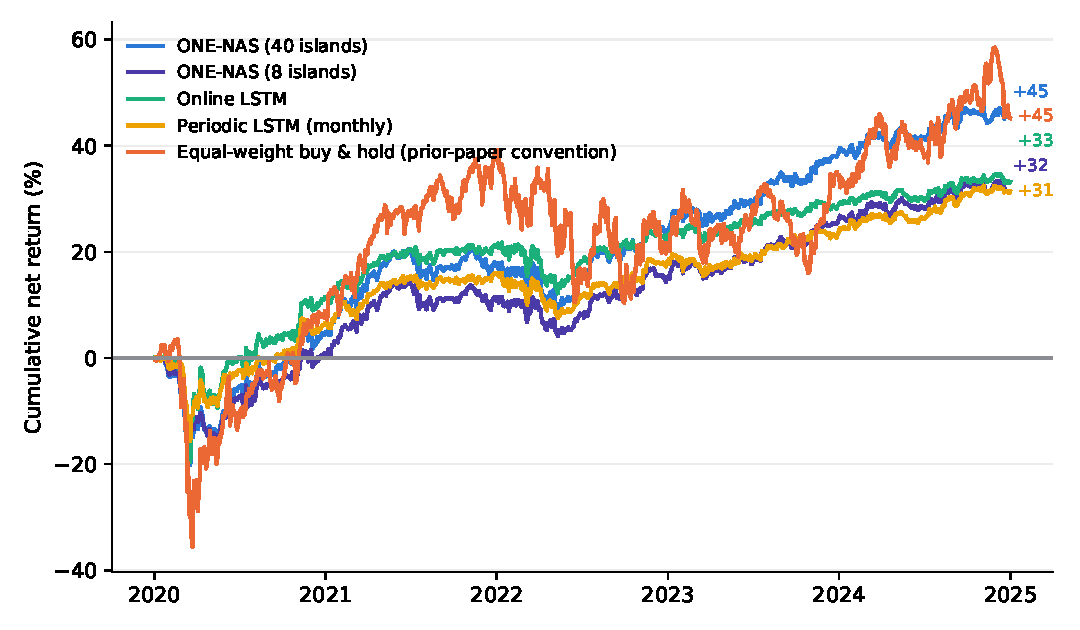
\includegraphics[width=\linewidth]{net_curves.pdf}
\caption{Cumulative net return, 2022--2024 (books restarted at window
start). Buy-and-hold follows the prior paper's benchmark convention.}
\label{fig:curves}
\end{figure}

\begin{table}[h]
\centering
\begin{threeparttable}
\caption{Prediction rule, within-run paired: single global-best genome
vs.\ island-champion rank-mean ensemble from the same runs (sleeves book).
Net \% / Sharpe; $\Delta$ = ensemble $-$ single, paired $t$ over seeds.}
\label{tab:m1}
\begin{tabular}{llrrrr}
\toprule
Fleet & Window & Single & Ensemble & $\Delta$net ($t$) & $\Delta$Sharpe ($t$) \\
\midrule
40 isl.\ ($n{=}10$) & 2022--24 & $+4.5$ / $0.21$  & $+27.5$ / $0.87$ & $+23.0$ $(18.2)$ & $+0.66$ $(14.7)$ \\
40 isl.\ ($n{=}10$) & 2020--24 & $+2.7$ / $0.08$  & $+45.6$ / $0.68$ & $+42.9$ $(14.6)$ & $+0.60$ $(13.4)$ \\
8 isl.\ ($n{=}10$)  & 2022--24 & $+8.3$ / $0.33$  & $+20.5$ / $0.70$ & $+12.2$ $(6.7)$  & $+0.37$ $(5.8)$ \\
8 isl.\ ($n{=}10$)  & 2020--24 & $+12.0$ / $0.21$ & $+32.1$ / $0.52$ & $+20.1$ $(5.5)$  & $+0.30$ $(5.3)$ \\
\midrule
8 isl.\ ($n{=}5$)\tnote{a}  & 2016--19 & $+16.3$ / $0.56$ & $+26.0$ / $0.92$ & $+9.7$ $(5.2)$   & $+0.36$ $(4.5)$ \\
40 isl.\ ($n{=}5$)\tnote{a} & 2016--19 & $+8.9$ / $0.30$  & $+36.7$ / $1.22$ & $+27.8$ $(7.5)$  & $+0.92$ $(6.6)$ \\
\bottomrule
\end{tabular}
\begin{tablenotes}\footnotesize
\item[a] Replication on the 2016--2019 tuning-span fleets.
\end{tablenotes}
\end{threeparttable}
\end{table}

\begin{figure}[h]
\centering
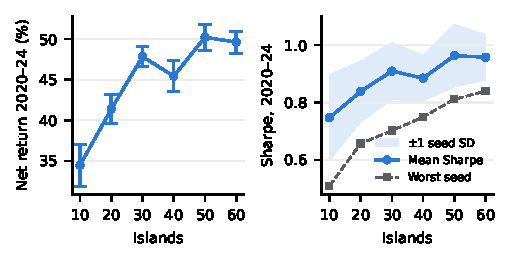
\includegraphics[width=\linewidth]{islands_scaling.pdf}
\caption{Performance vs.\ island count (2020--2024, registered sleeves
book; 10 seeds $\times$ 4 panels at every width). Left: pooled net return
(mean $\pm$ SE). Right: Sharpe --- mean with $\pm$1 seed-SD band, and the
worst seed. Return and Sharpe climb steeply to about 30 islands and then
sit on a plateau ($+45$ to $+50$ net, Sharpe $0.88$--$0.96$) whose widths
are not separable at this replication; the worst seed improves
monotonically across the whole range ($0.51 \to 0.84$) while the seed SD
falls ($0.149 \to 0.079$), so width keeps buying reliability after it
stops buying mean return. The 40-island setting was fixed on the
2016--2019 tuning span before this curve was measured; the nominally
higher 50- and 60-island cells are eval-span measurements and are not
adopted.}
\label{fig:islands}
\end{figure}

\begin{table}[h]
\centering
\begin{threeparttable}
\caption{Paired significance for the 2022--2024 window table: within-cell
difference in net return between ONE-NAS (40 islands) and each other arm,
over the (panel, seed) cells the two share.}
\label{tab:paired}
\begin{tabular}{lrr}
\toprule
Comparison & $\Delta$net & paired $t$ \\
\midrule
vs.\ ONE-NAS (8 isl.)            & $+7.0$  & $3.49$ \\
vs.\ Online LSTM                 & $+16.2$ & $7.32$ \\
vs.\ Online GRU                  & $+15.8$ & $6.59$ \\
vs.\ Periodic LSTM (monthly)     & $+12.7$ & $6.66$ \\
vs.\ Online AR\tnote{a}          & $+34.9$ & $2.22$ \\
\bottomrule
\end{tabular}
\begin{tablenotes}\footnotesize
\item Every comparison is over all 40 (panel, seed) cells unless noted.
Buy \& hold trades once and is not seed-paired, so no paired test is
reported against it.
\item[a] Deterministic; one run per panel, so $n{=}4$.
\end{tablenotes}
\end{threeparttable}
\end{table}

\begin{table}[h]
\centering
\begin{threeparttable}
\caption{Cost sensitivity: net return (\%) on 2022--2024 as the realised
per-name transaction cost is scaled by the stated multiple. The
$1\times$ column is the sleeves-book column of the window table.}
\label{tab:costs}
\begin{tabular}{lrrrrr}
\toprule
Arm & $1\times$ & $2\times$ & $3\times$ & $5\times$ & B/E\tnote{a} \\
\midrule
ONE-NAS (40 isl.)            & $+27.5$ & $+24.7$ & $+21.8$ & $+16.0$ & $10.6\times$ \\
ONE-NAS (8 isl.)             & $+20.5$ & $+17.4$ & $+14.4$ & $+8.2$  & $7.7\times$ \\
Periodic LSTM (monthly)      & $+14.8$ & $+11.4$ & $+8.0$  & $+1.2$  & $5.4\times$ \\
Online GRU                   & $+11.7$ & $+8.3$  & $+4.9$  & $-1.8$  & $4.5\times$ \\
Online LSTM                  & $+11.3$ & $+8.1$  & $+4.9$  & $-1.5$  & $4.5\times$ \\
Online AR                    & $-3.3$  & $-6.0$  & $-8.8$  & $-14.2$ & --- \\
\bottomrule
\end{tabular}
\begin{tablenotes}\footnotesize
\item Scaling multiplies the realised per-name cost, so the
cross-sectional shape of costs is preserved and wide-spread names stay
the expensive ones.
\item[a] Break-even: the cost multiple at which net return reaches zero.
\end{tablenotes}
\end{threeparttable}
\end{table}

\begin{table}[h]
\centering
\caption{Factor-adjusted alphas: pooled daily book returns regressed on
Fama--French three factors plus momentum, 2020--2024, Newey--West lag 10.}
\label{tab:alphas}
\begin{tabular}{lrrrr}
\toprule
Arm & $\alpha$ (bps/day) & $\alpha$ (\%/yr) & NW $t$ & Mkt.\ beta \\
\midrule
ONE-NAS (40 islands)     & $+3.15$ & $+7.9$ & $+2.14$ & $+0.120$ \\
ONE-NAS (8 islands)      & $+2.17$ & $+5.5$ & $+1.76$ & $+0.096$ \\
Periodic LSTM (monthly)  & $+2.15$ & $+5.4$ & $+1.78$ & $+0.079$ \\
Online LSTM              & $+2.08$ & $+5.2$ & $+1.59$ & $+0.130$ \\
Online GRU               & $+1.52$ & $+3.8$ & $+1.35$ & $+0.119$ \\
Online AR                & $-1.35$ & $-3.4$ & $-1.05$ & $+0.007$ \\
\bottomrule
\end{tabular}
\end{table}

\begin{table}[h]
\centering
\caption{Ensemble diversity mechanism: measured member rank IC, pairwise
member prediction correlation $\rho$, measured ensemble IC, and the
equicorrelated averaging prediction $m\sqrt{N/(1+(N-1)\rho)}$.}
\label{tab:diversity}
\begin{tabular}{lccccc}
\toprule
Fleet & $N$ & $\rho$ & Member IC & Ensemble IC & Predicted \\
\midrule
8 isl., 2020--24  & 8  & 0.216 & $+0.0064$ & $+0.0110$ & $+0.0114$ \\
40 isl., 2020--24 & 40 & 0.172 & $+0.0058$ & $+0.0128$ & $+0.0132$ \\
8 isl., 2016--19  & 8  & 0.190 & $+0.0071$ & $+0.0132$ & $+0.0132$ \\
40 isl., 2016--19 & 40 & 0.187 & $+0.0078$ & $+0.0166$ & $+0.0171$ \\
\bottomrule
\end{tabular}
\end{table}

\begin{table}[h]
\centering
\begin{threeparttable}
\caption{Ensembling gain (ensemble $-$ single champion, within-run, net \%
on 2016--2019) inside every trained hyperparameter configuration; positive
in 16/16 cells.}
\label{tab:invariance}
\begin{tabular}{lr@{\qquad}lr}
\toprule
Configuration & $\Delta$net & Configuration & $\Delta$net \\
\midrule
C0 (registered primary) & $+3.9$  & NTS 600            & $+12.8$ \\
Select: IC-gated        & $+0.5$  & Rounds 2           & $+11.0$ \\
Select: IC              & $+2.8$  & PER $\alpha$ 0.4   & $+4.0$  \\
Target: 5-day CS        & $+4.5$  & PER $\alpha$ 0.8   & $+11.7$ \\
5-day CS + IC-gated     & $+1.8$  & PER $\lambda{\times}3$ & $+20.6$ \\
Elite 5 / gen 10        & $+9.6$  & BP epochs 20       & $+12.5$ \\
Elite 5 / gen 15        & $+11.1$ & Repop.\ 25         & $+7.0$  \\
Repop.\ 100             & $+9.6$  & PER off (uniform)  & $+9.3$  \\
\bottomrule
\end{tabular}
\begin{tablenotes}\footnotesize
\item Mean $+8.3$; $n{=}6$ runs per cell (2 panels $\times$ 3 seeds).
\end{tablenotes}
\end{threeparttable}
\end{table}

\begin{table}[h]
\centering
\caption{Online continuity: pooled net (\%) on 2022--2024, frozen 8-island
configuration.}
\label{tab:continuity}
\begin{tabular}{lr}
\toprule
Population evolving online since 2020-01 & $+26.5$ \\
Cold start at 2022-01                     & $+12.3$ \\
\bottomrule
\end{tabular}
\end{table}

\begin{table}[h]
\centering
\caption{ONE-NAS hyperparameter settings (selected on 2016--2019
validation data, disjoint from the evaluation span). Replay sampling
ablated: PER vs.\ uniform shows no advantage on the tuning objective
($\Delta$IC $-0.0024$, $t{=}-1.9$).}
\label{tab:hps}
\begin{tabular}{ll}
\toprule
Hyperparameter & Value \\
\midrule
Islands & 40 (headline); 8 (registered primary) \\
Elite population per island & 8 \\
Generated genomes per island per generation & 5 \\
Repopulation frequency & every 50 generations \\
Selection metric & validation MSE \\
Prediction rule & rank-mean ensemble of island champions \\
Target & 1-day cross-sectional rank-normal return \\
Sequence length / window step / validation sets & 40 / 5 / 5 \\
Training subsequences per genome & 2000 \\
Backpropagation epochs per genome & 10 \\
Replay (PER) $\alpha$, $\lambda$, $\epsilon$ & 0.6, 0.007, $10^{-8}$ \\
Rounds per generation & 1 \\
Node-type library & simple, UGRNN, MGU, GRU, $\Delta$-RNN, LSTM \\
Mutation / intra- / inter-island crossover & 0.7 / 0.2 / 0.1 (framework defaults) \\
Warm-up generations & 50 \\
\bottomrule
\end{tabular}
\end{table}
